% !TeX document-id = {4983ff03-2248-4cb5-947e-a4cb90d994a7}
% Magic commands to enable write18 for automating inkscape-to-latex workflow
% !TeX TXS-program:compile = txs:///pdflatex/[--shell-escape]

\documentclass[11pt, parskip=half*,twoside=false]{scrbook}
\usepackage{todonotes}
\usepackage{natbib}
%\usepackage[utf8]{inputenc}
\usepackage[hidelinks]{hyperref}
\usepackage[UKenglish]{babel}
\usepackage[nottoc,notlot,notlof]{tocbibind}
\usepackage[UKenglish]{datetime}
\usepackage{graphicx}
\graphicspath{{./images/}}
\usepackage[mode=buildnew]{standalone} % requires -shell-escape

\newdateformat{monthyear}{%
	\monthname[\THEMONTH] \THEYEAR}

% Commands required for using the Bath-Harvard citation standard
\newcommand*{\urlprefix}{Available from: }
\newcommand*{\urldateprefix}{Accessed }
\bibliographystyle{bathx}

% No indents in references
\setlength\bibhang{0pt}
% This package allows linebreaks in URLs, fixing a problem with long URLs in the References
\usepackage{xurl}




\RedeclareSectionCommand[
runin = true,
beforeskip = 0.5\baselineskip,
afterskip = -1em]
{paragraph}

\renewcaptionname{UKenglish}{\bibname}{References}             %Bibliography

% Set up acronyms
\usepackage[toc, nogroupskip, nonumberlist, nopostdot]{glossaries}
\usepackage{glossary-mcols}
\makenoidxglossaries
\setacronymstyle{long-short}
\loadglsentries{gls_defns}
\glsfindwidesttoplevelname
\setglossarystyle{super}

%\usepackage{pgfplots}
\usepackage{pgfgantt}
\usepackage{lscape}
\usepackage{pdfpages}
%
%\usepackage[edges,linguistics]{forest}
%\usetikzlibrary{arrows.meta}
%

\usepackage[noabbrev]{cleveref}

%opening
\title{Low-Cost Attentiveness Detection Systems}
\author{Thomas M. S. Smith}
\subtitle{A literature review and project plan submitted to the University of Bath in partial fulfilment of the requirements for the award of MSc in Robotics and Autonomous Engineering}
\publishers{Department of Electronic \& Electrical Engineering \\ University of Bath}
\monthyear

\begin{document}

\maketitle

\frontmatter


\includepdf{declaration}
%\chapter*{Declaration}
%
%This literature review and project plan is submitted to The University of Bath in accordance with the requirements of the degree of Master of Science in Robotics and Autonomous Systems, in the Department of Electrical and Electronic Engineering. No portion of the work in this document has been submitted in support of an application for any other degree or qualification of this or any other university or institution of learning. Except where specifically acknowledged, it is the work of the author.
%
%\vskip 2cm
%\noindent\begin{tabular}{@{}p{0.5\textwidth}p{0.5\textwidth}@{}}
%	\dotfill                         & \dotfill\\
%	Thomas Smith              & Date\\
%\end{tabular} 


\addchap{Abstract}

Driver inattention is a leading cause of road traffic collisions resulting in avoidable injuries, deaths, and economic cost.
The development and adoption of autonomous vehicles has the potential to reduce these impacts, but also introduce additional driver inattention challenges. This work reviews a wide range of driver attentiveness monitoring systems proposed in the literature, with the aim of identifying gaps and opportunities for further development of such systems.

The non-contact detection of physiological signals is a well explored problem in the context of healthcare, with proposed methods including the use of radar based vital sign monitoring and \glsdesc{rppg}. A review of these methods is conducted to assess potential to adapt and adopt methods from healthcare for the problem of driver attentiveness monitoring.

Building on the literature review, a project plan has been proposed. The aims and objectives of the project have been elaborated and specifications, milestones and deliverables have been defined.

\tableofcontents

\printnoidxglossary[sort=letter, title={List of Abbreviations}]

\mainmatter

\chapter{Introduction} \label{ch:intro}
%\glsresetall


%This chapter presents an introduction to the project and to this report. Present the motivation and background for the project, before laying out the structure of the report.  \todo{improve slightly}

\section{Motivation} \label{sec:motive}

%\paragraph{Notes}
%\begin{itemize}
%	\item Road traffic collision casualty numbers
%	\item Driver inattention and distraction as contributor to road traffic collisions
%	\item Increasing adoption of level 2 and 3 ADAS systems, still require full driver attention
%	\item Possible application in level 4 and 5 systems
%	\item Vital sign monitoring as part of attentiveness detection, and value of non-contact vital sign monitoring in healthcare settings
%	\item Highlight opportunities for translation from healthcare to this application
%	\item Briefly discuss challenges of transition (different environment, different subject status)
%\end{itemize}

Driver inattention is one of the leading causes of \glspl{rtc} \citep{petridouHumanFactorsCausation2000,youngDriverDistraction2007,olsonDriverDistractionCommercial2009}. The increasing adoption of driving automation systems has the potential to improve road safety and reduce the incidence and severity of \glspl{rtc} \citep{favaroExaminingAccidentReports2017} but the introduction of such systems does present additional challenges for driver inattention. A number of collisions involving automated driving systems have been reported where the driver appears to have failed to provide the required level of supervision to the automated system, see for example \citep{ntsbCollisionSportUtility2019,ntsbCollisionCarOperating2019}. Existing methods of monitoring driver attentiveness in production vehicles, such as Tesla's monitoring of steering wheel torque, are easily defeated by a user and so do not provide sufficient protection. The large contribution to \glspl{rtc} made by driver inattention, coupled with the increasing adoption of automated driving systems, are the primary motivation for this work. A robust driver attentiveness monitoring system may reduce accidents in manual driving by encouraging drivers to, for example, rest when fatigued, and may also facilitate the wider and safer adoption of automated driving systems which will in turn reduce \gls{rtc} instances. 

A common approach for driver attentiveness monitoring is based on the measurement of driver vital signs, with \gls{ncvs} monitoring being particularly suited to the automotive environment. This presents an opportunity to benefit from and to contribute to advances in the field of healthcare in \gls{ncvs} monitoring. The continuous monitoring of the vital signs of the circulatory and respiratory systems is important for the monitoring and treating of many diseases in a variety settings, from the home to the ward. However it is impractical, and in some cases impossible, to use contact based measurements, motivating the development of various \gls{ncvs} monitoring approaches. 


\section{Report Structure} \label{sec:struct}
\todo{Double check matches actual structure}
The remainder of this document is structured as follows. \Cref{ch:litreview} presents a review of the literature relevant to the problem of driver attentiveness monitoring. \Cref{sec:distraction} presents definitions and a taxonomy of driver inattention before discussing the different levels of autonomous vehicles. A review of the literature specific to driver inattention is presented in \cref{ssec:approaches}, with accompanying analysis in \cref{ssec:analysis}.  \Cref{sec:vital_sign} considers the literature related to non-contact vital sign measurements in a healthcare setting, highlighting vision and radar based approaches.  

\Cref{ch:plan} proposes a project plan for the development and test of a proof-of-concept driver attentiveness monitoring system using radar based non-contact vital sign measurements, before \cref{ch:conc} concludes the document.

%
%\todo{Write out in long form}
%Brief overview of the document structure, as follows:
%\begin{itemize}
%	\item Literature review:
%	\begin{itemize}
%		\item Driver distraction and inattention:
%		\begin{itemize}
%			\item Why it matters
%			\item Define taxonomy
%			\item Present approaches from previous works:
%			\begin{itemize}
%				\item Driving behaviour measures
%				\item Driver physiological measures (focus)
%			\end{itemize}
%			\item Detailed discussion of some key approaches:
%			\begin{itemize}
%				\item Relevance
%				\item Strengths, weaknesses
%				\item Reliability
%				\item Accuracy
%			\end{itemize}
%		\end{itemize}
%		\item Vital sign monitoring:
%		\begin{itemize}
%			\item Brief overview of major vital signs used in healthcare (personal and clinical settings)
%			\item Brief overview of monitoring approaches used in personal and healthcare settings
%			\item Focus on non-contact vital sign monitoring:
%			\begin{itemize}
%				\item Vision based (e.g. Lifelight)
%				\item Radar based
%				\item Other?
%			\end{itemize}
%		\end{itemize}
%		\item Gaps and Opportunities
%		\item Discussion/Analysis:
%			\begin{itemize}
%				\item Draw links between driver distraction/awareness and healthcare setting
%				\item Highlight promising approaches
%				\item Highlight challenges and gaps
%				\item Conclude literature review
%			\end{itemize}
%		\end{itemize} 
%	\item Project plan:
%	\begin{itemize}
%		\item Aims and objectives
%		\item Specification
%		\item Milestones and deliverables
%	\end{itemize}
%\end{itemize}


\chapter{Literature Review} \label{ch:litreview}
%\glsresetall
This chapter comprises a review of the literature on driver attentiveness monitoring and vital sign measurements. Driver inattention is considered first, with definitions and a taxonomy of inattention providing a starting point for the review, before considering autonomous vehicle applications which can represent a particularly challenging context for driver inattention. Approaches for driver monitoring in the literature are presented and discussed before vital sign monitoring in healthcare is considered.

\section{Driver inattention monitoring} \label{sec:distraction}
\subsection{Overview and definitions} \label{ssec:overview}
%\paragraph{notes}
%\begin{itemize}
%	\item Highlight why driver attentiveness matters, introduce SAE autonomous vehicle levels, examples of when it goes wrong
%	\item Discuss and define driver distraction and inattention
%	\item Present taxonomy (either from \citep{reganDriverDistractionDriver2011} or specific to this work, prefer from source)
%\end{itemize}
%
%\paragraph{content}

In this work the term driver inattention is used according to the definition of \citet{reganDriverDistractionDriver2011} to mean `insufficient, or no attention, to activities critical for safe driving'. This inattention can stem from a number of different sources including fatigue and external distractions. The potential sources of inattention have implications for the design of an attentiveness monitoring system\textemdash an appropriate input signal detect fatigue induced inattention is likely to differ from a signal for distraction.  \citet{reganDriverDistractionDriver2011} identify five categories of driver inattention, resulting in the taxonomy presented in \cref{fig:taxonomy_inattention}. A brief discussion of these five categories is given here with the intention of identifying whether a category lends itself to monitoring via a driver attentiveness system. 

\begin{figure}[h]
	\centering
	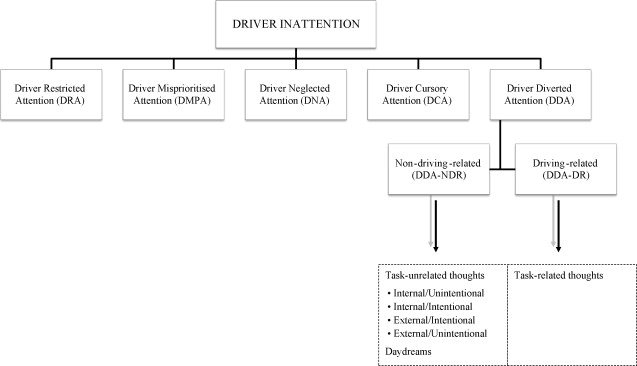
\includegraphics[width=\textwidth]{driver_inattention_taxonomy} 
	\caption{Taxonomy of driver inattention. Reproduced AS-IS with permission from \citep{reganDriverDistractionDriver2011}.}
	\label{fig:taxonomy_inattention}
\end{figure}

\paragraph{\gls{dra}}caused by biological factors, such as fatigue. 

\paragraph{\gls{dmpa}} the driver incorrectly pays too much attention to one area of the driving task at the expense of a second equally or more important task. For example when merging lanes the driver needs to consider traffic in front and behind them and in both lanes, which can be challenging to achieve simultaneously.

\paragraph{\gls{dna}} the driver's mental model of the driving task causes them to neglect information which is critical to the task. An example would be a driver failing to detect and interpret a new traffic sign or change to the road layout on a route that are very familiar with. 

\paragraph{\gls{dca}} caused by cursory attention being applied to critical elements of the driver task, for example a glance in the rear-view mirror without fully processing the scene. 

\paragraph{\gls{dda}} encompasses driver distractions, and is defined by \citet{reganDriverDistractionDriver2011} as `the diversion of attention away from activities critical for safe driving towards a competing activity'. Such diversion can be related to the driving task or non-driving related, and may be manual, visual, cognitive, or a combination of the above, in nature. Changing gear in a manual car may be considered as a driving related manual distraction, as the driver is required to take one hand off the steering wheel. Writing a text message on a mobile telephone would be a non-driving related manual, visual and cognitive distraction. 

No literature was found that detected \gls{dmpa}, \gls{dna} or \gls{dca}, and it is not clear how one would monitor or detect these forms of inattention. The causes and consequences of these types of inattention can however be mitigated through \gls{adas} systems such as automatic emergency braking or blind-spot warnings. As such, these forms of inattention are not considered further in this work.

\gls{dra} and \gls{dda} are widely considered in the literature, and are more relevant for autonomous vehicle applications as discussed next. Theses forms of inattention are the focus of this work.

\subsection{Automated driving systems}
\todo{Needs tweaking and checking}
As \glspl{ads} become more common and more advanced, the issue of driver inattention is likely to become even more critical. One particular area of concern is partially-autonomous vehicles, where the driver is still required to monitor and react to the environment while the \gls{ads} is performing certain driving tasks.  In \citep{J3016_201806} SAE International introduced a taxonomy and definitions for six levels of driving automation which is widely used in the discussion of autonomous vehicles. A summary of the six levels is shown in \cref{fig:av_levels}. These six levels of autonomy are based on four main factors which differentiate between whether the (human) driver or the automated system is responsible for certain tasks: 

\begin{enumerate}
	\item Who is performing primary driving actions (lateral and longitudinal control) 
	\item Who is detecting and responding to obstacles and events
	\item Who is the fallback should the automated system fail or reach an area outside of its operational design domain
	\item The extent and any limitations on the operational design domain\textemdash the environment(s) in which the automated system is designed to operate
\end{enumerate}

\begin{figure}[h]
	\centering
	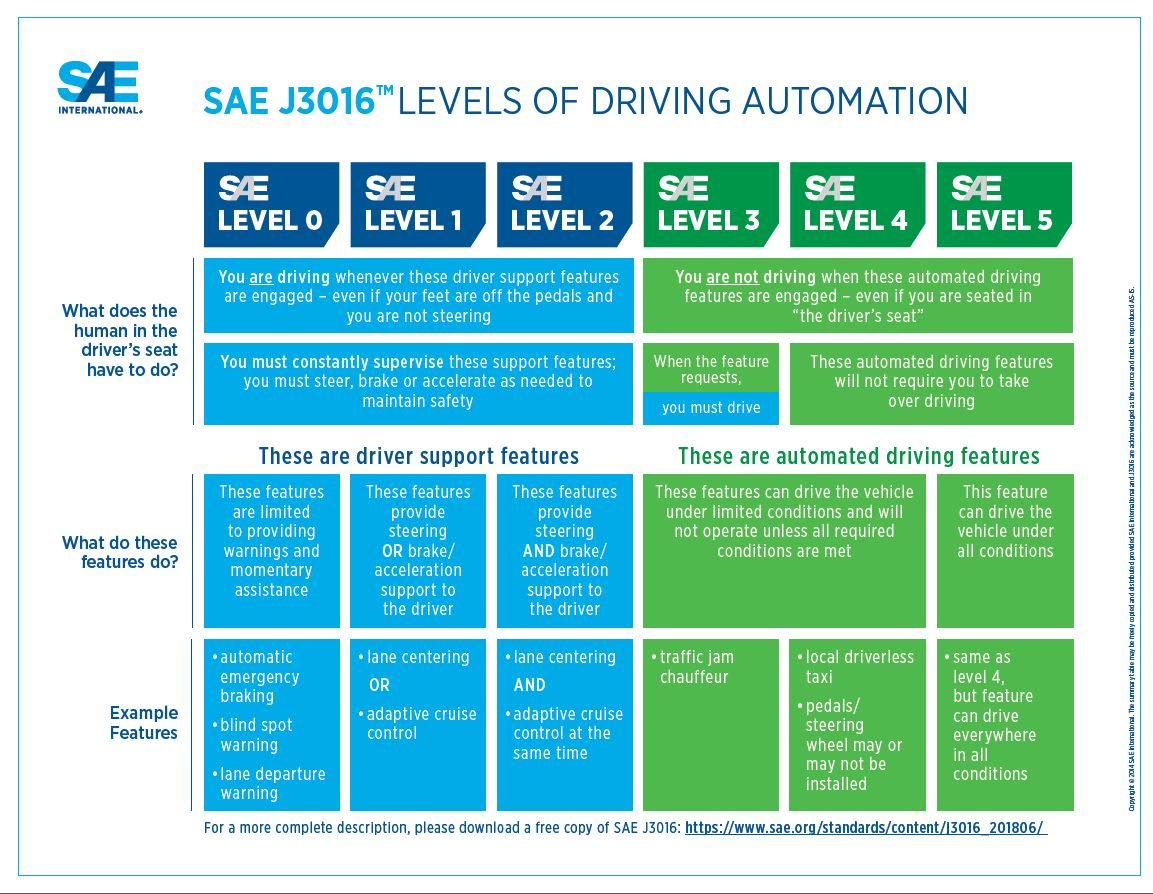
\includegraphics[width=\textwidth]{sae_av_levels} 
	\caption{Levels of driving automation. Reproduced AS-IS with permission from \citet{J3016_201806}.}
	\label{fig:av_levels}
\end{figure}

A brief discussion of these levels of driving automation follows, highlighting the importance of driver attentiveness monitoring at the different levels of automation. 

SAE level 0 systems feature no driving automation. The human driver is always controlling the lateral (steering) and longitudinal (acceleration and braking) motion of the vehicle, and detecting and responding to obstacles and events during the driving task. There are exceptions for \gls{adas} such as automatic emergency braking, but these are not considered further here as they do not relate to the issue of driver attentiveness. Driver inattention and distraction is a concern in level 0 systems, with a review reporting driver inattention or distraction as a cause in approximately one quarter of \glspl{rtc} in the United States \citep{youngDriverDistraction2007}. A system with the capability to detect inattention or distraction could provide the driver with visual, audible or tactile alerts and warnings may increase driver attention or cause the driver to take a rest stop, and so reduce the likelihood of an \gls{rtc}.

In SAE levels 1 and 2 the human driver of the vehicle is always considered to be driving the vehicle, even if lateral and/or longitudinal control (steering and/or braking) is performed by the \gls{ads}. A level 1 system provides steering \emph{or} accelerator and brake support to the human driver, while a level 2 system can perform both tasks. The Tesla vehicles involved in the \glspl{rtc} in \cref{sec:motive} were SAE level 2 vehicles with the Tesla \gls{ads} system, `Autopilot' engaged. 

An SAE level 3 autonomous vehicle is capable of driving the vehicle under limited conditions, and the human is not considered to be the driver while the level 3 \gls{ads} is engaged. However the human driver must take back control of the driving task when requested to do so by the \gls{ads}. It is hopefully apparent that there are significant concerns and issues around driver distraction and inattention in level 1, 2 and 3 \gls{ads}, and these are areas where a low cost driver attentiveness monitoring system will offer benefits in safety and ....  \citet{teohWhatNameDrivers2020} reports that drivers consider many actions to be safe while a level 2 system is in operation, they're wrong, particularly bad for Autopilot.

\citet{goncalvesDrowsinessConditionalAutomation2016} experimentally investigated passive fatigue caused by underloading a driver when autonomous systems are used. The majority of subjects reported high levels of drowsiness within 15 minutes, and a decrease in performance when responding to take over requests was found.

Levels 4 and 5 can both be considered fully autonomous and the human driver is never expected or required to take control of the driving task. Level 4 is restricted to operate in limited circumstances, while level 5 automation can drive under all conditions. Driver attentiveness monitoring is not directly relevant to level 4 and 5 systems, however the closely related task of driver mood monitoring may be beneficial, allowing the \gls{ads} to tailor the vehicle ambience, driving route and style to the human occupants' current mood.

In addition to all of this, a driver monitoring system which includes monitoring of vital signs may provide valuable information to emergency response and accident investigation teams (driver is alive but deteriorating, driver was healthy before \gls{rtc} vs driver had heart attack before \gls{rtc}). 

\subsection{Approaches for monitoring inattention} \label{ssec:approaches}
A number of approaches for driver attentiveness monitoring have been proposed in the literature, using a variety of measured signals to detect the different forms of driver inattention, \gls{dra} and \gls{dda}, introduced previously. Due to the different causes and symptoms of \gls{dra} and \gls{dda} some approaches are better suited to detecting one or the other. Monitoring approaches can either be categorised according to the form(s) of driver inattention they are best suited to monitoring or according the measures that are used to assess attentiveness. This section considers the relevant literature, starting with those that investigate \gls{dda} detection before considering \gls{dra} monitoring and, finally, works that monitor both forms of driver inattention. 

\subsubsection{Driver Distracted Attention monitoring}
\citet{wollmerOnlineDriverDistraction2011} detect driver attention from head movements and driving behaviour signals with a \gls{lstm} \gls{rnn}. The model is trained and tested using a real world driving dataset with non-driving related distraction tasks such as operating the in-vehicle information systems. This type of task involves visual, manual and cognitive distractions. The input signals for the model were head position, steering wheel angle, throttle position, speed, heading and lane position. Two approaches were considered. In the first, raw \emph{low-level} signals are used as inputs to the model, while the second approach uses statistical functions over a number of frames to calculate \emph{functionals} as the input. F1 scores were up to $96.0\%$ for the binary classification problem using functionals, and as low as $38.1\%$ for the six class problem using low level signals. In general the functional inputs resulted in higher accuracies than the low level signals, and increasing the number of classification classes reduced the accuracy. The authors compared their results to a standard \gls{rnn} and a \gls{svm} based approach and reported higher accuracy using the \gls{lstm} method in all cases.

The use of an \gls{lstm} in this work was motivated by the temporal nature of driver distraction and the input signals. \Glspl{rnn} in general and \glspl{lstm} in particular are well suited to pattern matching of time-series data.

\citet{liangHybridBayesianNetwork2014} use a similar set of inputs and a layered algorithm to detect cognitive distraction. The algorithm comprises a \gls{dbn} and a supervised clustering layer, a combination which aims to reduce the computational complexity of \gls{dbn} approaches while maintaining the interpretability of these methods.

The algorithm uses driver eye tracking and driving behaviours as inputs. Driving behaviour is measured as the standard deviation of both steering wheel angle and lane position, as well as steering error. Steering error is a metric of steering smoothness proposed by the authors, and is calculated by comparing the actual steering wheel angle to a steering angle predicted by a second-order Taylor expansion. 

The dataset used for training and testing was collected in a driving simulator, with the subjects being exposed to auditory cognitive distraction. The authors compare their algorithm to both \gls{dbn} and \gls{svm} models, reporting comparable performance but with reduced training and prediction times, and improved interpretability.

\citet{aksjonovDetectionEvaluationDriver2019} implemented a rule based expert system using fuzzy logic for measuring driver distraction. An \gls{ann} is trained to predict the lane position and speed based on speed limits and turn radius. This is compared to actual lane position and speed with a fuzzy logic control to predict a percentage measure of driver distraction. The use of non-linear regression to predict a numeric value of driver distraction is an interesting distinction of this work.

The system was tested in driver-in-the-loop experiments in a driving simulator, with the participant replying to a text message while driving. Qualitatively the predicted values of driver distraction align with the periods in which the driver was distracted, although it is not clear if the absolute value of the prediction corresponds to the actual level of distraction. A limitation of this work is that it relies on the driver first completing the driving route with no distractions and as accurately as possible to train the \gls{ann}. This is likely to limit the application of this system in the real world vehicles.

 \citet{dingInattentiveDrivingBehavior2019} use a \gls{fmcw} radar used to detect driver inattention. They highlight the privacy concerns of cameras in the cockpit of a vehicle, and suggest that a radar based system would be more acceptable to consumers. Seven driver behaviours associated with inattention were investigated. Radar measurements were converted into time-Doppler spectrograms and range-Doppler trajectories and inattention is predicted from these features using a classifier. A range of machine learning methods were tested as classifiers, with a Bagged Trees approach having the highest average accuracy across the seven investigated driver behaviours, achieving $94.8\%$, $93.3\%$ and $95.6\%$ average accuracy when using time-Doppler, range-Doppler, and combined features respectively. The authors experimented with 5.8~GHz and 24~Ghz radars, reporting that the resolution of the 5.8~Ghz radar was too low for this approach.
 

\subsubsection{Driver Restricted Attention monitoring}
The works considered here aim to monitor \gls{dra} in the form of fatigue or drowsiness.
 
\citet{jungDriverFatigueDrowsiness2014} used an \gls{ecg} sensor embedded in steering wheel to detect \gls{hrv}\textemdash the variation of the time interval between heart beats. \gls{hrv} can be used to evaluate the function of the \gls{ans} which can indicate normal, fatigued and drowsy states. \gls{hrv} is analysed in both the time domain and the frequency domain. Time domain \gls{hrv} is based on beat-to-beat intervals while frequency based \gls{hrv} is a measure of the power spectral density found using parametric \gls{fft}.

Testing of the system is limited, with only two test subjects over a two hour driving test, and results are reported qualitatively. More robust testing and reporting would be required before such a system was used in production. Additionally, the signal is measured using contact based sensors, requiring the driver to have their hands correctly positioned on the wheel. 
 
\citet{zhangAutomatedDetectionDriver2014} used a variety of entropy and complexity measures of \gls{eeg}, \gls{emg} and \gls{eog} signals for the real-time detection of fatigue. An \gls{ann} is trained to classify fatigue in one of four levels using the complexity measures. The accuracy of estimation is between $96.5\%$ and $99.5\%$. A limitation of this work is that \gls{eeg}, \gls{emg} and \gls{eog} signals are measured using contact-based sensors with complex and expensive equipment (electrodes placed on occiput, eyelids, and neck). These are unlikely to be accepted by consumers in a personal vehicle.

\citet{tsuchiyaHeartbeatDetectionTechnology2020} placed a 24~GHz radar in the driver seat back to measure heart rate. A heartbeat generates a small displacement of the body surface which is detected by the radar system. However  respiration and body movements fall in the same band, making it difficult to extract heartbeat. Additionally, vibrations from driving cause noise to be superimposed over the sensor signal reducing the signal-to-noise ration of the signal. The authors proposed measurement algorithm comprising various band-pass filters and Fourier transforms to filter the noise from the signal. The system was evaluated via in-car testing with an \gls{ecg} as ground truth. The algorithm improved accuracy during driving compared to the authors' previous method but still gave poor equivalence to the \gls{ecg} ground truth. This highlights the challenges of operating in a driving environment and the importance of real-word testing where possible. 

%\citet{liDetectionDriverDrowsiness2013} wavelet transform of \gls{hrv} signals measured using \gls{ppg} with a \gls{svm} classifier with categories alert and drowsy. Incorporated into an application which will find a nearby rest location if fatigue is detected. A $1^\text{st}$ order differential operation is used to filter movement induced noise from the \gls{hrv} time series data, which is then decomposed into nine wavelet levels before an \gls{svm} is used to classify the level of fatigue. The system was tested with four participants in a driving simulator. The accuracy of the classification of the drivers' fatigue (as alert of drowsy) was 95\%.

\citet{yuDriverDrowsinessDetection2019} use four different models to detect fatigue: representation learning, scene understanding, feature fusion, and fatigue detection. The representation learning model uses a 3D \gls{cnn} that allows for a sequence of video frames to be used as an input to the \gls{cnn}, and outputs a spatio-temporal representation of a scene. This representation is passed through a scene understanding model which interprets key features of the scene, including illumination and head, mouth and eye conditions. The output of the scene understanding model is combined with the scene representation in a fusion model, before a detection model classifies the driver as fatigued or alert. The combined model is resilient to variations in scene composition, such as the wearing or removal of glasses, and variation in light conditions. 
 
The system was trained and tested using the \gls{nthu} Drowsy Driver Detection video dataset \citep{wengDriverDrowsinessDetection2017} which consists of over nine hours of video data of 36 subjects performing simulated driving tasks while making various facial expressions in response to external requests. A potential issue with this dataset is that the facial expressions and other displays of fatigue are being simulated by the participants by them acting as if they were fatigued. It is likely that the facial expressions and behaviour of an individual experiences real fatigue will differ from these simulated expressions. However this dataset does allow researchers to demonstrate the feasibility of a given approach, even if further training and testing is required in real-world conditions.

The average classification accuracy was $76.2\%$ and was consistently more accurate than alternative approaches tested on the same dataset. Although the final accuracy reported is low compared to some other methods considered here, it is difficult to directly compare works which are assessed under different conditions and using different datasets. In addition the dataset used in this work includes a number of challenging scenarios, such as direct sunlight, night and the wearing and removal of glasses which are not considered directly in other works.

A 3D \gls{cnn} was also used to detect driver fatigue by \citet{gaoEEGBasedSpatioTemporal2019}, but with an  \gls{eeg} signal as input. Data for training and testing is from a driving simulator with eight subjects. Two class classification accuracy was $97.37\%$, higher than all eight comparison methods considered by the authors.

\citet{fuDynamicDriverFatigue2016} applied a \gls{hmm} to biological signals for fatigue detection based on \gls{eeg}, \gls{emg} and respiration rate signals. Their system was tested during real-world driving with 12 professional driver. The drivers self-reported their state as alert, mildly fatigued or fatigued and these reports were used as the ground truth for comparison of the system. Qualitatively the \gls{hmm} predictions of fatigue aligned with the self-reported fatigue levels. The use of simple self-reported measures as ground truth is a weakness of this work.

\citet{zhouPredictingDriverFatigue2021} focus on explainable fatigue prediction. They performed a series of experiments in a driving simulator, with the subject performing a simple driving task before an \gls{ads} took over the driving task, with the subject supervising the \gls{ads} system but completing no additional tasks. This tended to induce passive fatigue in the participants as discussed by \citep{goncalvesDrowsinessConditionalAutomation2016}. \gls{perclos} was used as the ground truth signal for fatigue. Measures used for the prediction model were related to heart rate and respiratory rate, as well as \gls{ecg}, steering wheel torque and angle, and driver posture. The most important measures according to SHAP value were \gls{hr} (averaged over 60 seconds), \gls{hrv} and breathing rate (averaged over 60 seconds). Interesting \gls{ecg} was reported as the second lowest important measure - \gls{ecg} is commonly used for fatigue detection and is a heart rate based signal. It may be that a similar effect to that reported by \citet{wollmerOnlineDriverDistraction2011}, where the outputs of statistical analysis of raw signals made better inputs to the model then the raw signals themselves.
 
Two approaches were found that aim to monitor both \gls{dra} and \gls{dda}. \citet{crayeMultiModalDriverFatigue2016} implemented a multi-modal system making use of audio, vision, depth map, heart rate, and steering wheel and pedal positions. Their systems is able to detect fatigue and distraction with $98.4\%$ and $90.5\%$ accuracy respectively. Input signals are processed by three modules (vision, audio, other) with each module producing an independent estimation of driver fatigue and distraction using \glspl{hmm}. The outputs of each module are fused with contextual information in a Bayesian network. The system separately processes driver fatigue and distraction and can be enable or disabled individually. \Glspl{hmm} are used due to the temporal nature of the problem space and dataset.

The dataset used is gathered from eight subjects in a driving simulator. Drivers simulated the symptoms of fatigue (yawning, closing their eyes) and were also tasked with completing a number of distracting tasks during the experiment. Distraction was classified as one of either two or five classes, with the two class classification being more accurate.

\citet{duaAutoRateHowAttentive2019} developed an approach using a \gls{cnn} and \gls{gru} for spatio-temporal representation of visual sensory input, using the front facing camera of a windscreen mounted smartphone. Their dataset comprised 2,900 unique video segments, each 10~seconds long and covering 30 drivers performing real-world driving tasks in a large city. Each video segment was rated on a five point scale by human annotators. 

A number of pre-trained \glspl{cnn} are used to extract both generic features and specific facial features from the input frames. The outputs of both the generic and specific networks are combined using \glspl{lstm} so that the temporal nature of both fatigue and distraction are considered. The system was tested on 782 unseen videos with an accuracy of $70\%$ compared to the human annotators.

\subsection{Discussion} \label{ssec:analysis}
A wide range of different input signals have been considered in the literature. \Cref{fig:taxonomy_measures} presents a taxonomy of these signals, grouped by the type of measure. It is clear that different types of signal are preferred for monitoring \gls{dra} or \gls{dda}. This effect can be seen in \cref{fig:summary} which presents a summary of the input signals by inattention type considered. Driver physiological measures are primarily used for \gls{dra} type inattention such as fatigue, while driving and driver behaviour measures are predominately used to detect driver distraction. No \gls{dda} detection method uses driver physiological signals. 

\begin{figure}[h]
	\centering
	\includestandalone{inattention_monitoring_taxonomy}
	\caption{Taxonomy of driver inattention measures.}
	\label{fig:taxonomy_measures}
\end{figure}

This highlights a key challenge in this field, as driving behaviour methods are of limited value in level 2 and 3 autonomous vehicles, as the \gls{ads} is in control of lateral and longitudinal motion for extended periods of time. As such methods that use driver behaviour or physiological measures are preferred.

Many of the driver physiological measures discussed in this review are commonly measured with contact based sensors. This approach is not likely to be acceptable to consumers in personal vehicles, and the sensors themselves are expensive and require careful positioning to get accurate readings. Non-contact physiological measurement approaches are therefore likely to be more promising for driver fatigue assessment, and are considered in more detail in the following section.

\begin{landscape}	
	\begin{figure}[b]
		\centering
		\includestandalone[width=1.4\textwidth]{summary_graph}
		\caption{A summary of measurement inputs identified in this review, categorised by the type of driver inattention detected in the work.}
		\label{fig:summary}
	\end{figure}
\end{landscape}	


\section{Non-contact vital sign monitoring} \label{sec:vital_sign}
%\glsresetall
Many of the driver inattention detection methods discussed in \cref{ssec:approaches} use driver vital signs as an input. The acquisition of driver vital signs poses a number of challenges, including the expense and complexity of the sensing equipment, and the discomfort and distraction caused by contact-based sensors. These challenges also exist in healthcare settings, and so a significant body of work investigates \gls{ncvs} monitoring devices in a clinical setting. This section considers existing literature which make use of vision and radar inputs as these align with the automotive setting.

\subsection{Radar}
The first reported use of microwave signals for the non-invasive measurement of respiration is by \citet{linNoninvasiveMicrowaveMeasurement1975}, who made microwave measurements of respiratory movement of a rabbit and a human subject. Since then a number of radar based approaches have been proposed to measure respiration and heart rates. Radar based vital sign monitoring relies on measuring the Doppler shift of the radar signal which is caused by movement of the chest wall from breathing and heart pumping. A wide number of different frequencies have been used in the literature, as shown in \cref{fig:radar_freqs}. The majority of works summarised in \cref{fig:radar_freqs} use the 24~GHz frequency band, but the \gls{uwb} at 24~Ghz is being phased out and will not be available after January 1, 2022 \citep{ramasubramanianMovingLegacy242018}, motivating the exploration of other frequencies. In particular, higher frequencies , and so reduced wavelengths, have the following advantages: 
\begin{itemize}
	\item Improved range resolution
	\item Reduced device form factor
	\item Improved directionality and therefore increased range
\end{itemize}

\begin{figure}[h]
	\centering
	\includestandalone[width=\textwidth]{radar_summary}
%	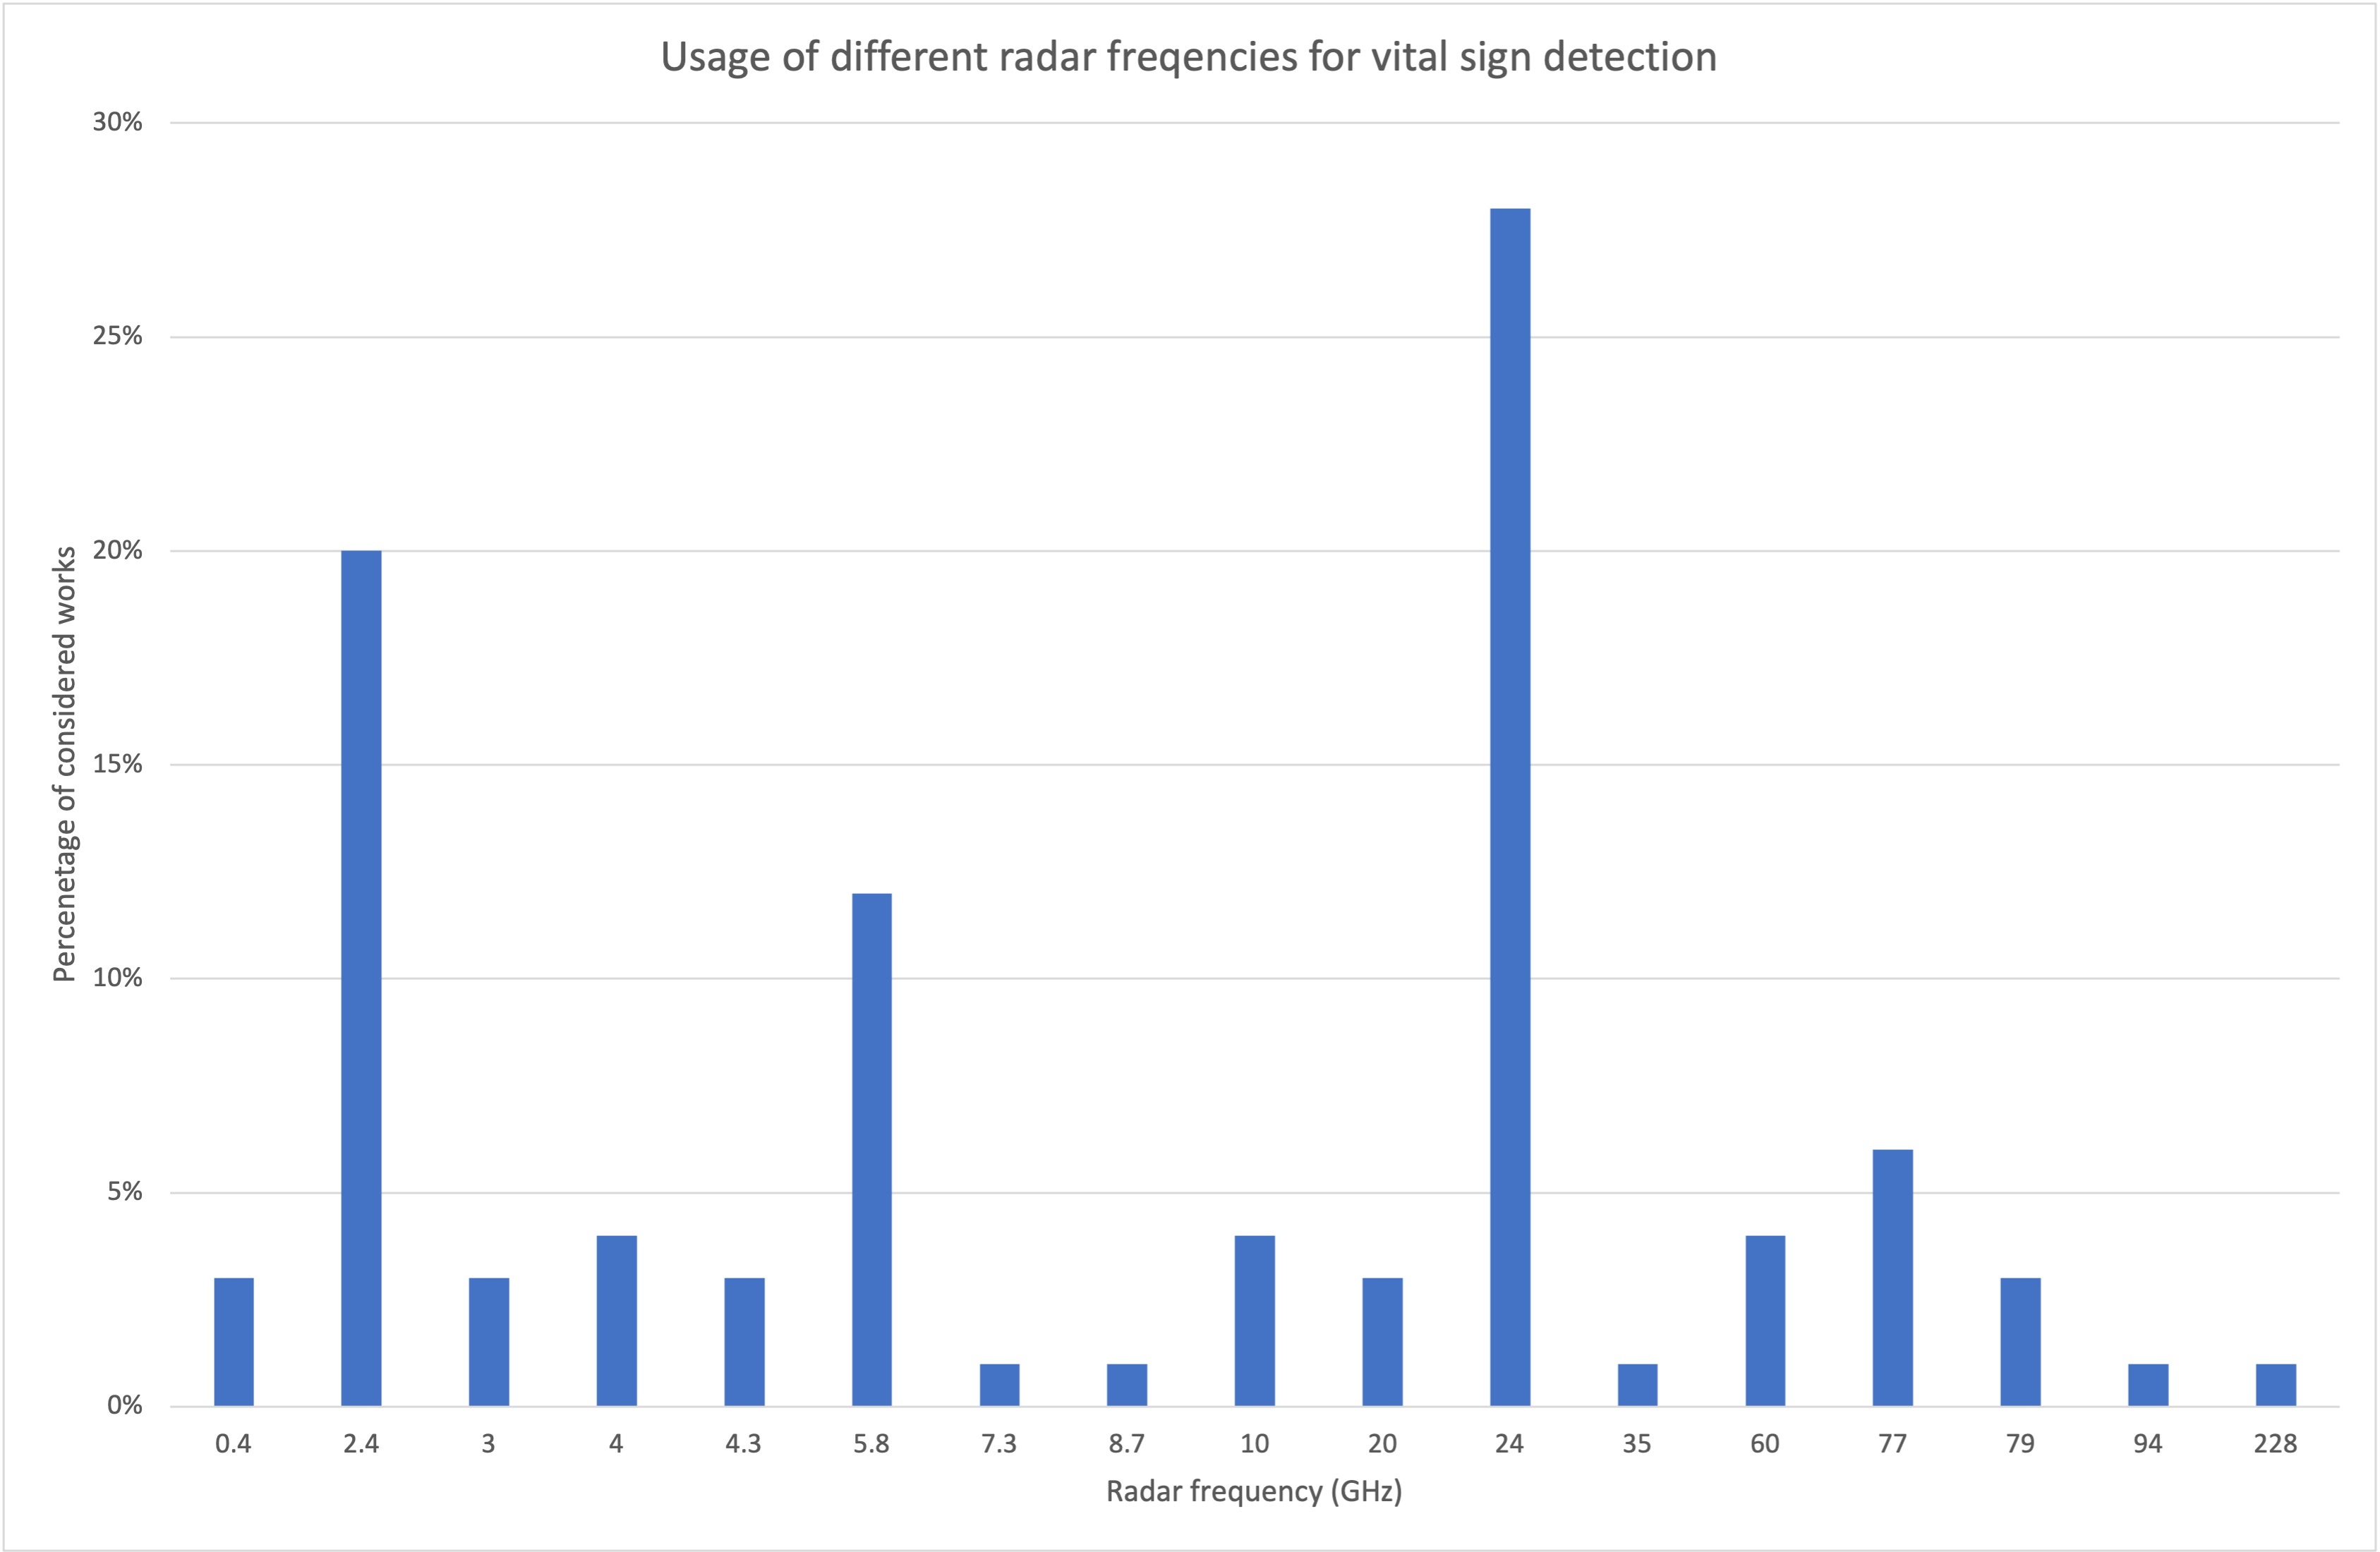
\includegraphics[width=0.95\textwidth]{radar_frequencies} 
	\caption{A summary of the radar frequencies used in a variety of works. Data from \citet{singhMultiResidentNonContactVital2021}}.
	\label{fig:radar_freqs}
\end{figure}

Two recent examples of radar based heart rate measurements are introduced here.  \citet{willAdvancedTemplateMatching2017} use a 24~GHz \gls{cw} radar with an advanced template matching algorithm for instantaneous heartbeat detection. Five different types of heartbeat signal templates are used, each defined by six features. When comparing the interbeat interval to a reference \gls{ecg} signal the \gls{rmse} was 18.0~ms, compared to 68.2~ms with a previous template matching approach. The same authors apply a hidden semi-Markov model to radar signals to detect heart sounds \citep{willRadarBasedHeartSound2018}. \gls{ecg}and \gls{pcg} measurements are used as ground truth for heartbeat and heart sound detection respectively. Heart sounds detected using this method were strongly correlated to heartbeats measured using \gls{ecg}, with an F-score of $92.22\pm 2.07 \%$.

\subsection{Vision}
Vision based monitoring systems are based on \gls{rppg}, which uses a camera to measure the changes in blood volume in blood vessels under the skin. This method is similar to traditional \gls{ppg} but does not rely on a specific light source or contact with the subject. \citet{verkruysseRemotePlethysmographicImaging2008} were the first to demonstrate that \gls{ppg} signals can be acquired remotely under ambient lighting conditions using a consumer grade camera pointed at the subject's face. The patient's face and a background \gls{roi} are identified. Pixel values in each colour channel are spatially averaged to improve \gls{snr} at the expense of spatial resolution. The authors reported that motion artefacts during measurements disrupt readings, and that the green channel shows best signal for \gls{hr} detection.

{\citet{tarassenkoNoncontactVideobasedVital2014} extended on the above work, incorporating an auto-regressive model to filter out noise caused by artificial light flicker. \citet{villarroelContinuousNoncontactVital2014} consider a  neonatal intensive care setting, using the same techniques to monitor \gls{hr}, \gls{rr}, and \gls{spo2} of 30 pre-term infants in incubators. They reported sensitivity to large changes in ambient light conditions, subject movement and covered skin impacted readings. The authors found that, for an absolute error of 4~\gls{bpm}, there is no significant difference in the measurement discrepancies for the vision based method and the \gls{ppg} or \gls{ecg} methods when compared to the discrepancy between the \gls{ppg} and \gls{ecg} measures themselves. In a continuation of this work, \citet{villarroelNonContactVitalSign2017} use a video camera to estimate heart rate, respiratory rate and changes in peripheral oxygen saturation in a different healthcare setting\textemdash patients undergoing dialysis. Two \gls{ppg} sensors are used at to different locations on the subject as a reference signal for \gls{hr} and \gls{spo2}. \gls{ecg} and a chest belt were used for \gls{rr} reference signals. The system was tested over 61 dialysis sessions, totalling 219.8 hours of video. The mean absolute error of the \gls{hr}, \gls{rr} and \gls{spo2} estimations were 2.8~\gls{bpm}, 2.1~\gls{bpm} and $2.5\%$ respectively. Note that the errors between the two reference pulse oximeters were 1.87~\gls{bpm} and $0.97\%$ for \gls{hr} and \gls{spo2} respectively, which is comparable to the errors in the estimated signals.  A problem with this approach is that a large number of the video sessions recorded were not suitable as inputs due to patient and camera movements, obstructed views of the patients face and medical interventions. 

This technology is being commercialised by Lifelight \citep{ximlimitedLifelightXimLimited2021} for use in consultations and telehealth settings and a number of clinical trials have been completed or are in progress. Results to date are  promising and the commercialisation in a clinical setting highlights the possibility of \gls{rppg} methods for driver attentiveness detection.

\section{Gaps and opportunities}
A wide variety of works covering driver inattention and healthcare have been considered. This section discusses gaps and opportunities identified from the review.

It is apparent that there are no definitive, objective, measures for \gls{dra} or \gls{dda} which presents a challenge when developing and comparing driver attentiveness monitoring systems. As most fatigue and distraction measures are subjective and self-reported, such as the Karolinska Sleepiness Scale \citep{kaidaValidationKarolinskaSleepiness2006}, it is challenging to attain ground truth data for training and testing. This also makes any comparison of the accuracy of different methods invalid if they are based on different ground truths. 

Additionally, many studies force subjects to act the symptoms of fatigue or to complete a distracting task while in a simulated environment. This is likely due to the ethical and practical challenges of capturing data of fatigued and distracted drivers in the real world but does present challenges. It is unlikely that an individual pretending to yawn or drift off to sleep will display the same behaviours and physiological signs as in reality. Practical and ethical considerations are also likely the driver for most studies being performed in driving simulators, and with low numbers of subjects. Real world testing with suitably large numbers of subjects will be required to validate any method before real world adoption.

Driving behaviour is widely used as an input for driver attentiveness monitoring. While this is valuable and useful as an input in level 0 systems, the value starts to deteriorates with level 1 \gls{ads} and they are not usable for level 2 and level 3 systems, where both lateral and longitudinal control is by the \gls{ads}. This means that alternative measures are needed for driver distraction monitoring. 

Many of the approaches that detect driver fatigue require invasive\textemdash in the context of driving a car\textemdash measurement devices. These are not viable in real world due to driver comfort and the risk of causing driver distraction in their own right. Some physiological measures are only available through such methods, including \gls{eeg} and \gls{emg} but other measures can be detected remotely. Some opportunities are presented by the review of \gls{ncvs} in healthcare. \gls{rppg} is a promising technique which has not been thoroughly explored for driver fatigue detection \citep{sikanderDriverFatigueDetection2019}. Radar based systems have received a lot of attention for \gls{ncvs} detection in healthcare \citep{sikanderDriverFatigueDetection2019} but less so in driver attentiveness monitoring. One interesting use of radar in driverless attentiveness monitoring is the distraction detection approach of \citet{dingInattentiveDrivingBehavior2019}, one of the few distraction monitoring approaches that does not rely on driving behaviour signals. This opens up the potential for a radar based system to detect both \gls{dra} and \gls{dda} forms of driver inattention.


%\section{Discussion}
%\paragraph{notes}
%Draw links between driver distraction/awareness and healthcare setting,highlight promising approaches and directions, and existing challenges to overcome. Draw the literature review to a close by summarising review and findings. Tie into project direction
%
%\begin{itemize}
%	\item Discuss sensors / measures as applicable to vehicle environment \citep{crayeMultiModalDriverFatigue2016} as a good starting point
%	\item Discuss values of different measures (binary vs. classifier vs. regression)
%	\item Discuss relative importance / ease of measure fatigue vs. distraction
%	\item Discuss cross-over from driver attentiveness to healthcare setting (both directions)
%	\item Audio isn't used much and is interesting to consider, but is it feasible when you consider radio / podcast / music etc.?
%\end{itemize}
%
%

\chapter{Project Plan} \label{ch:plan}
%\glsresetall
This chapter presents the objectives, specification and plan for the project, informed by the literature review of \cref{ch:litreview}.

\section{Aims and objectives}
This project aims to design, develop and validate a proof-of-concept low-cost driver attentiveness monitoring system suitable for the automotive environment.

The literature review highlights the useful of non-contact vital sign monitoring for driver fatigue detection, and suggests opportunities to adopt and influence techniques used in healthcare. It is also apparent that driver distraction is an important form of driver inattention, but one that is hard to monitor without driving behaviour measures. The method proposed by \citet{dingInattentiveDrivingBehavior2019} is one of the few distraction monitoring approaches that does not rely on driving behaviour signals, instead making use of radar. As radar is also a viable measurement signal for driver physiological signals a radar based system may be able to monitor both driver distraction and driver fatigue.  As such radar is identified as the primary source for this work. Additionally, vision has the potential to detect both distraction and vital signs, although with additional privacy concerns. As such, vision will be considered as a secondary source where appropriate.

The objectives of this project, in ascending order of complexity, are:
\begin{itemize}
	\item The accurate and reliable measurement of cardiovascular measures from a radar signal.
	\item The accurate and reliable measurement of respiration rate from a radar signal.
	\item The accurate and reliable measurement of cardiovascular measures using \gls{rppg}.
	\item The accurate and reliable measurement of respiration rate using \gls{rppg}.
	\item Detection, classification and/or measurement of subject fatigue using a radar signal.
	\item Detection and/or classification of subject distraction using a radar signal.
\end{itemize}

\section{Milestones and deliverables}

A plan for the completion of the proposed project has been prepared and is shown as a Gantt chart in \cref{fig:gantt}. The first milestone is the completed planning of data collection experiments, which requires defining requirements for the dataset and identifying the hardware and software components necessary for data collection, before producing a plan for conducting data collection experiments. Next, the hardware and software components required for data collection are assembled, before data collection experiments are performed. The intention is for experiments to involve a number of subjects from different demographics, although this is subject to any COVID restrictions in place at the time.  

The design, development and testing of algorithms has been structured as a series of sprints, were each sprint will deliver a viable algorithm that fulfils at least part of the relevant specification. This ensures progress towards the project objectives is being made while allowing for iterative development of the system. A total of three sprints are planned. The methods and findings of each sprint are documented and reported before moving onto the next sprint. This encourages reflection on progress to date so that approaches used in subsequent sprints are informed by findings to date.  

Report drafting starts at the end of the first development sprint, reflecting the intention for sprint documentation and reporting to be incorporated into the final thesis. A thesis structure will be agreed as part of the drafting process and the project finishes with the an oral presentation and submission of the thesis.

No specific contingency line has been included in the plan, but the impact of exams and COVID restrictions have been considered at each line item. Additionally, the adoption of sprints facilitates the removal or addition of sprints as time pressures mandate. 

\ganttset{calendar week text={\small{\startday/\startmonth}}}
\begin{landscape}	
	\begin{figure}

		%	\section{Timeline}	\label{app:Gantt}
		\begin{ganttchart}[
				hgrid,
				vgrid={*{6}{draw=none},dotted},
				x unit = 1.2mm,
				y unit chart = 5.4mm,
				time slot format=isodate,
				title height=1,
				milestone/.append style={xscale=2.25},
				]{2021-05-03}{2021-09-12}
				\gantttitlecalendar[]{month=shortname} \\
				\gantttitlecalendar[title height=1.5,title label node/.append style={rotate=90}]{week=18}\\
				\gantttitle[title/.style={opacity=0}]{}{0}\\ % invisible title to make room for previous higher line
				\ganttbar{Revision}{2021-05-03}{2021-05-28} \\
				\ganttmilestone{Exams}{2021-05-18}
				\ganttmilestone{}{2021-05-21} \\
				\ganttgroup{Data collection}{2021-05-10}{2021-06-27} \\
				\ganttbar{Dataset requirements}{2021-05-10}{2021-05-30} \\
				\ganttbar{Experiment planning}{2021-05-17}{2021-06-06} \\
				\ganttmilestone{Experiment plan}{2021-06-06} \\
				\ganttbar{Rig build}{2021-06-07}{2021-06-13} \\
				\ganttmilestone{Ready for experiment}{2021-06-13} \\
				\ganttbar{Collect data}{2021-06-14}{2021-06-27} \\
				\ganttgroup{Development Sprints}{2021-06-21}{2021-07-17} 
				\ganttgroup{}{2021-07-19}{2021-08-07}
				\ganttgroup{}{2021-08-09}{2021-08-29} \\
				\ganttbar{Implement algorithm}{2021-06-21}{2021-07-11}
					\ganttbar{}{2021-07-19}{2021-08-01} 
					\ganttbar{}{2021-08-09}{2021-08-22} \\
				\ganttbar{Train \& test algorithm}{2021-07-12}{2021-07-18}
					\ganttbar{}{2021-08-02}{2021-08-08}
					\ganttbar{}{2021-08-23}{2021-08-29} \\
				\ganttbar{Documentation}{2021-07-16}{2021-07-18}
					\ganttbar{}{2021-08-06}{2021-08-08}
					\ganttbar{}{2021-08-27}{2021-08-29} \\
				\ganttbar{Report drafting}{2021-07-19}{2021-09-09} \\
				\ganttmilestone{Thesis structure agreed}{2021-08-15} \\				
				\ganttmilestone{Report first draft}{2021-08-29} \\
				\ganttmilestone{Report final draft}{2021-09-05} \\
				\ganttmilestone{Oral presentation}{2021-09-08} \\
				\ganttmilestone{Thesis complete}{2021-09-10} \\				
			\end{ganttchart}
	
			\caption{A Gantt chart showing the plan for completion of the proposed project. Each column marked by dashed lines represents one week.}
			\label{fig:gantt}	
	\end{figure}	

\end{landscape}

\chapter{Conclusion} \label{ch:conc}

This report has reviewed the literature to identify a range of driver attentiveness monitoring systems. The importance of driver attention has been highlighted, particularly with regard to recent and future advances in autonomous driving systems, and a taxonomy and definition for driver inattention has been presented. Methods identified in the literature primarily seek to monitor driver fatigue or driver distraction, very few methods are capable of monitoring both forms of inattention. The primary input signals for driver distraction monitoring are driving behaviour measures which will not be applicable to level 2 and 3 autonomous vehicles. As such, an alternative driver distraction monitoring approach is required. Driver fatigue is primarily detected by driver behaviour and physiological signals, often using contact based sensors which are not viable in a commercial setting. 

The non-contact detection of physiological signals is a well explored problem in the context of healthcare, with proposed methods including the use of radar based vital sign monitoring and \gls{rppg}. The adoption of these approaches for driver attentiveness monitoring will be considered in future work.

Building on the literature review, a project plan has been proposed. The aims and objectives of the project have been elaborated and specifications, milestones and deliverables have been defined.

%\nocite{*}
\bibliography{references}

\end{document}